\documentclass[tikz,border=2pt]{standalone}
\usepackage{amsmath,amssymb}
\usepackage{tikz}
\usetikzlibrary{arrows.meta}

\begin{document}
% Maximise f on the constraint curve h(x) = c: walking along the curve, f stops increasing
% exactly where a level set of f touches the curve, i.e. where the gradients are parallel.
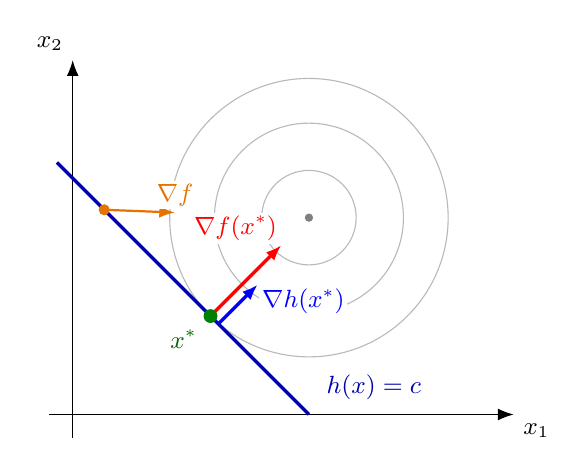
\begin{tikzpicture}[every node/.style={font=\small}, >={Latex[length=2mm]}, lab/.style={font=\small, fill=white, inner sep=1pt}]
	\foreach \r in {0.6,1.2,1.768} {\draw[gray!55] (3,2.5) circle (\r);}
	\fill[gray] (3,2.5) circle (1.5pt);
	\draw[->] (-0.3,0) -- (5.6,0) node[below right] {$x_1$};
	\draw[->] (0,-0.3) -- (0,4.5) node[above left] {$x_2$};
	\draw[blue!70!black, very thick] (3.0,0) -- (-0.2,3.2);
	\node[blue!70!black, anchor=south west, font=\small] at (3.1,0.06) {$h(x)=c$};
	\fill[orange!90!black] (0.4,2.6) circle (2pt);
	\draw[->, orange!90!black, thick] (0.4,2.6) -- (1.3,2.565) node[above, lab, yshift=1pt] {$\nabla f$};
	\draw[->, red, very thick] (1.75,1.25) -- (2.65,2.15) node[above left, lab] {$\nabla f(x^\ast)$};
	\draw[->, blue, very thick] (1.85,1.15) -- (2.35,1.65) node[below right, lab] {$\nabla h(x^\ast)$};
	\fill[green!50!black] (1.75,1.25) circle (2.5pt);
	\node[green!40!black, anchor=north east, font=\small] at (1.7,1.2) {$x^\ast$};
\end{tikzpicture}
\end{document}
